\documentclass[table,dvipsnames,11pt,a4paper]{article}

\usepackage[utf8]{inputenc}
\usepackage{lmodern}
\usepackage{textcomp}
\usepackage{float}
\usepackage{tikz}
\usepackage[top=80pt,bottom=120pt,left=75pt,right=75pt]{geometry}
\usepackage{microtype}
\usepackage{graphicx}
\usepackage{listings}
\usepackage{subcaption}
\usepackage{parskip}
\usepackage{appendix}
\usepackage{bm}
\usepackage{amsmath}
\usepackage{amssymb}
\usepackage{xcolor}
\usepackage{relsize}
\usepackage{enumitem}
\usepackage{amsfonts}
\usepackage{textgreek}
\usepackage{booktabs}
\usepackage{array}
\usepackage{xfrac}
\usepackage[labelfont=bf,font=footnotesize]{caption}
\usepackage[hypertexnames=false,hidelinks]{hyperref}
\usepackage[noabbrev,nameinlink,capitalize,poorman]{cleveref}

\bibliographystyle{unsrt}

% \renewcommand{\thesection}{Task \arabic{section}}
\renewcommand{\thesubsection}{\arabic{subsection}}

\newcommand{\argmax}{\text{argmax}}
\newcommand{\rand}{\text{rand}}

\newcommand{\appendixA}{\hyperref[param_sweep_result_appendix]{Appendix A}}

\usetikzlibrary{matrix}
\usetikzlibrary{fit}
\usetikzlibrary{plotmarks}
\usetikzlibrary{positioning}
\usetikzlibrary{external}
\tikzexternalize[prefix=tikz/]

\setcounter{topnumber}{10}
\setcounter{bottomnumber}{10}
\setcounter{totalnumber}{10}
% \renewcommand{\floatpagefraction}{1}

\definecolor{coolgray}{rgb}{0.95,0.95,0.95}
\lstset{
	language=Python,
	backgroundcolor=\color{coolgray},
	tabsize=2,
	keywordstyle=\bfseries\color{OliveGreen},
	numbers=left,
	breakatwhitespace=true,
	captionpos=t,
	frame=single,
	basicstyle=\ttfamily\tiny,
	extendedchars=true,
	emphstyle=\color{Blue},
	showstringspaces=false,
	morekeywords={with, as},
	literate={✗}{X}1 {●}{o}1 {×}{$\times$}1 {→}{\textrightarrow}1 {↓}{\textdownarrow}1 {←}{\textleftarrow}1 {↑}{\textuparrow}1 {¡}{ }1,
}


\begin{document}

\begin{titlepage}
	\centering
	\includegraphics[width=\textwidth]{City\_logo} \\[4em]
	\begin{bfseries}
		\begin{Huge}
			Deep Reinforcement Learning \\[35pt]
			\textsl{Written Report}
		\end{Huge}
	\end{bfseries}
	\vfill{}
	\begin{LARGE}
		\begin{sffamily}
			Martin Fixman and Sean Lim \\
			Sean Lim and Martin Fixman \\
			2023/2024 Term \\
		\end{sffamily}
	\end{LARGE}
\end{titlepage}

\renewcommand{\thesection}{Basic Task}

\newcommand{\upa}{\mathlarger{\uparrow}}
\newcommand{\downa}{\mathlarger{\downarrow}}
\newcommand{\lefta}{\mathlarger{\leftarrow}}
\newcommand{\righta}{\mathlarger{\rightarrow}}

\section{Q Learning}

\subsection{Working Environment and State Transition and Reward Functions}

\begin{figure}[h]
	\begin{subfigure}{.49\textwidth}
		\centering
		\includegraphics[width=170pt,height=125pt,draft]{snow_puzzle_original.png}
		\caption{Original puzzle}
	\end{subfigure}
	\begin{subfigure}{.49\textwidth}
		\centering
		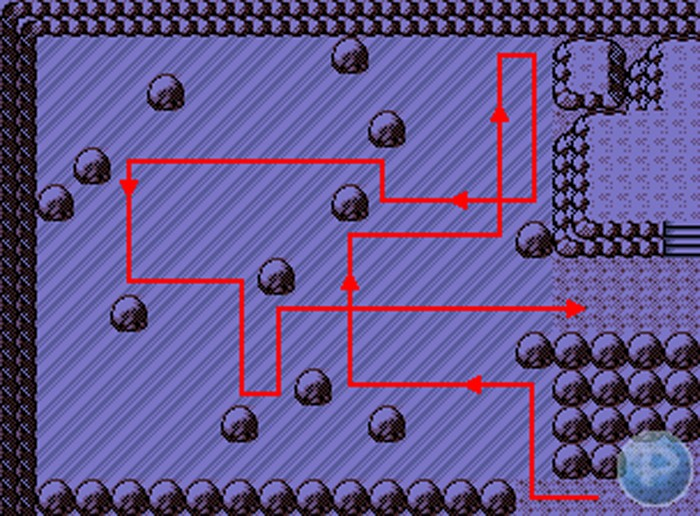
\includegraphics[height=125pt]{snow_2.png}
		\caption{Puzzle solution}
	\end{subfigure}
	\caption{An example of a Pokémon Ice puzzle}
	\label{large_map}
\end{figure}

In this task we present a solver of \emph{Pokémon Ice Puzzles}, a kind of ice puzzle where the player starts at a certain position $s$ and has the objective to reach its objective $e$ in as few steps as possible.

At each turn, the player can do one of four movements: $\{\upa, \downa, \lefta, \righta\}$.
As the environment is ice, when the user walks in any direction is slips on the ice and keeps going on the same direction until hitting a rock or the edge.

\newcommand{\coor}[2]{\left\langle #1, #2 \right\rangle}
\newcommand{\yx}{\coor{y}{x}}
\newcommand{\obs}{\mathcal{O}}
\newcommand{\state}{\mathcal{S}}
\newcommand{\reward}{\mathcal{R}}
The state function $\state$, along with the transition and reward functions $\mathcal{T}$ and $\reward$ can be defined as the following, where $\obs_{\yx}$ is true if and only if there is an obstacle on position $\yx$.
\begin{gather*}
	\state = \yx \qquad \mathcal{D} \in \left\{ \upa, \downa, \lefta, \righta \right\} \\
	\begin{aligned}
		&T_{\yx}\left(\upa\right) &= \coor{t + 1}{x} &&&\text{where } \obs_{\coor{t}{x}} \wedge \neg \obs_{\coor{q}{x}} \forall q \in \left(t, y\right) \\
		&T_{\yx}\left(\downa\right) &= \coor{t - 1}{x} &&&\text{where } \obs_{\coor{t}{x}} \wedge \neg \obs_{\coor{q}{x}} \forall q \in \left(y, t\right) \\
		&T_{\yx}\left(\lefta\right) &= \coor{y}{t + 1} &&&\text{where } \obs_{\coor{y}{t}} \wedge \neg \obs_{\coor{y}{q}} \forall q \in \left(t, x\right) \\
		&T_{\yx}\left(\righta\right) &= \coor{y}{t - 1} &&&\text{where } \obs_{\coor{y}{t}} \wedge \neg \obs_{\coor{y}{q}} \forall q \in \left(x, y\right)
	\end{aligned} \\
	\reward(\yx) = \begin{cases}
		100 & \text{if } e = \yx \\
		0 & \text{otherwise}
	\end{cases}
\end{gather*}

\subsection{Q Function}

This transition function allows us to define an iterative $Q$ function, which should be used to find the objective $Q^\pi$ function.
\begin{gather*}
	s \in \mathcal{S} \qquad a \in \mathcal{D} \\
	Q^{k + 1}(s, a) = \alpha \cdot \left( \reward( T( a, s ) ) + \gamma \cdot \max{Q^k(s, a)} \right) - Q^k(s, a)
\end{gather*}

\newpage{}
The probability next action $a$ is defined depending on the policy used, where $\pi^k(a \mid s)$ represents the probability of choosing action $a$ with state $s$ at point $k$.
\begin{gather*}
	\intertext{\textbf{\textepsilon-Greedy Policy}: choose the best policy with probability $\varepsilon$, randomly otherwise.}
	\pi^k(a \mid s) = 
		(1 - \varepsilon) \cdot \frac{1}{\mathcal{D}} + \varepsilon \cdot \begin{cases}
			1 & \text{if } a = \argmax_{a'} (Q^k(s, a')) \\
			0 & \text{otherwise}
		\end{cases} \\
	\intertext{\textbf{Bellman Policy}: choose policy using the softmax of the Q-value}
	\pi^k(a \mid s) = \frac{e^{Q^k(s, a)}}{\sum_{a' \in \mathcal{D}}{e^{Q^k(s, a')}}}
\end{gather*}

\subsection{Parameter sweep}
To find the best parameters, we run a parameter sweep on the map in \cref{large_map} for each combination of parameters in \cref{param_sweep_params}; this map is large enough to make it suitable for a parameter sweep.

\begin{table}[h]
	\scriptsize
	\centering
	\begin{tabular}{>{\bfseries}r | l l l l}
		\toprule
		Hyperparameter & \multicolumn{4}{c}{Values} \\
		\midrule
		Policy & \multicolumn{4}{l}{\begin{tabular}{l l}$\varepsilon$-Greedy & Bellman\end{tabular}} \\
		$\alpha$ & 0.1 & 0.5 & 0.7 & 0.9 \\
		$\gamma$ & 0.9 & 0.99 && \\
		$\varepsilon$ Decay Rate & 0.75 & 0.9 & 0.99 & \\
		\bottomrule
	\end{tabular}
	\caption{The parameter sweep considered every possible combination of these parameters.}
	\label{param_sweep_params}
\end{table}

Each combination was run 10 times until the Q matrix converged to a precision of $10^{-12}$ and results were averaged.
The final results, which contain the best parameters, can be found in \appendixA{}
Some interesting results can be found in \cref{param_sweep_interesting}.

\begin{table}[h]
	\scriptsize
	\centering
	\begin{tabular}{>{\bfseries}r r l r | r r r r}
		\toprule
		Policy & $\alpha$ & $\gamma$ & $\varepsilon$ Decay &
		E.\ to Conv & Best route & E.\ to Done & E.\ to Best \\
		\midrule
		\rowcolor{YellowGreen}
		\textepsilon{}-Greedy & 0.5  & 0.90  & 0.99 & 139 & 16.00 & 31.80  & 97 \\
		\textepsilon{}-Greedy & 0.9 & 0.90  & 0.90 & 51  & 16.80 & 12.00  & 26 \\
		\midrule
		Bellman & 0.2 & 0.90 & 0.75 & 666  & 16.20 &  82.70 &  224 \\
		Bellman & 0.9 & 0.90 & 0.99 & 126  & 17.40 &  37.30 &   86 \\
		Bellman & 0.7 & 0.90 & 0.75 & 205  & 17.60 &  48.70 &   58 \\
		\bottomrule
	\end{tabular}
	\caption{Some notable results taken from \appendixA{}.}
	\label{param_sweep_interesting}
\end{table}

We can observe the following.
\begin{itemize}
	\item The \textepsilon{}-Greedy policy converges faster and produces a significantly better result.
	\item Generally having high $\varepsilon$ Decay represents better results.
	\item There is a significant correlation between convergence speed and how good the solutions are.
\end{itemize}

We choose the parameter combination that converges the fastest between the ones that \emph{always} found the best solution; that's marked in \colorbox{YellowGreen}{green}.


\renewcommand{\thesection}{Advanced Task}
\section{Deep Ice Skating using Deep Q-Learning}
\subsection{Environment}
The environment used for the Basic Task is too basic to implement Deep Q Learning. Instead, we created a more complicated ice rink environment, taking inspiration from the  same concept of the environment used in the Basic Task.

The agent is now located in a circular ice skating rink dojo which contains non-integer locations.
They are also using real ice skates that cannot easily control turning velocity.
Instead, each agent can accelerate or deaccelerate their turning speed at each turn.
In addition to the turning restrictions, the agent must constantly go forward at a constant speed and cannot stop or slow down at any point.

For reference, \textbf{\cref{circle_plots}} shows the result of one of our models in the environment.

When skating, the state consists of 4 floating point values and the state has 3 different actions.

\begin{center}
	\begin{minipage}[t]{.48\textwidth}
		\begin{center}
			\textbf{States}
		\end{center}
		\begin{description}[noitemsep,style=nextline]
			\item[\bm{$y$}] The $y$ coordinate of the agent.
			\item[\bm{$x$}] The $x$ coordinate of the agent.
			\item[\bm{$\varphi$}] The current angular the agent is at.
			\item[\bm{$\theta$}] The current angular velocity.
		\end{description}
	\end{minipage}
	\begin{minipage}[t]{.48\textwidth}
		\begin{center}
			\textbf{Actions}
		\end{center}
		\begin{description}[noitemsep]
			\item[0. Turn Left] Decrease angular velocity.
			\item[1. Stay Put] Keep angular velocity.
			\item[2. Turn Right] Increase angular velocity.
		\end{description}
	\end{minipage}
\end{center}

An agent starts at a random point of the ice dojo facing at a random direction but not turning.
Its objective is to get to the centre as fast as possible.
This dojo is finite: if the agent goes far enough, it will fall off the flat earth and the game is terminated.

The state and transitions functions are defined in the following equation.
\newcommand{\statet}{\left< y, x, \varphi, \theta \right>}
\begin{gather*}
	\state = \statet \\
	\begin{aligned}
		y'(\state, a) &= y + \frac{1}{4} \sin(\varphi'(\state, a)) \\
		x'(\state, a) &= x + \frac{1}{4} \cos(\varphi'(\state, a)) \\
		\varphi'(\state, a) &= \varphi + \theta'(\state, a)
	\end{aligned}
	\qquad
	\theta'(\state, a)= \begin{cases}
		\theta^t - \frac{1}{10} \pi & \text{if } a = 0 \\
		\theta^t & \text{if } a = 1 \\
		\theta^t + \frac{1}{10} \pi & \text{if } a = 2
	\end{cases} \\[1ex]
	T(\state, a) = \left< y'(\state, a), x'(\state, a), \varphi'(\state, a), \theta'(\state, a) \right>
\end{gather*}

The reward function is defined to maximise the changes of an agent making it to the centre by, in addition to giving high scores for winning and low scores for losing, giving it a score depending on the distance to the centre.
\begin{equation*}
	\reward(\state) = \begin{cases}
		\phantom{+}1000 & \text{if } \sqrt{y^2 + x^2} \leq \text{min distance} \\
		-1000 & \text{if } \sqrt{y^2 + x^2} \geq \text{max distance} \\[1ex]
		-\sqrt{y^2 + x^2} & \text{otherwise}
	\end{cases}
\end{equation*}

Adding a reward that depends on the distance considerably improved training speed and precision of the Deep Q-network compared to just subtracting a constant each time.
Even though the results ``should'' be the same, subtracting the distance disincentives the agent from attempting bad solutions.

\newpage{}
\subsection{Implementation}
We implement a 3-layer Deep Q-network with hidden size set as a hyperparameter that's trained using an epsilon-greedy policy whose $\varepsilon$ value goes down linearly from a certain $\varepsilon$-start to 0.
The data used to train the model is accumulated and later randomly sampled from a large replay buffer.

The original network (target = DQN) produces good solutions if trained in large batch sizes for a large amount of episodes.
Frustratingly, it takes a very long time to even make ``passable'' solutions.

In order to improve these convergence time, we present two improvements that can be alternatively added to this model.


\subsection{Improvements}
For the improvements we have implemented two algorithms, mainly the target network method and the
Double-DQN method. Both of the methods vary slightly in the implementation algorithm, but may have
impacting results if implemented right.
\subsubsection{Target Network}
The target network method introduces a new variable called the target network. The target network is initialised as an exact copy of the main network otherwise used in the conventional DQN method, but instead of updating every timestep, the target network is instead updated every certain timesteps, denoted by the variable update frequency, hence causing the target network to always lag behind the main network in terms of training.
The target network in this method evaluates the action made by the main network, calculating the best action and its Q-values using the formula:
\begin{align*}
    Q_{\text{target}}(s, a ; \theta^{-}) = r + \gamma \max_{a'} Q(s', a' ; \theta^{-})
\end{align*}
Evaluating the actions of the main network using the target network aims to increase the stability of the
overall training of the agent.

\subsubsection{Double DQN}

The double-DQN method (DDQN) similarly utilises the target network used by the target method method, but it differs in the sense that instead of getting the best actions and its q-values like the aforementioned two methods, the DDQN method gets the best action through the main network, but calculates the q-values using the target network, using the following formula:
\begin{align*}
    Q^{\text{DDQN}}(s, a ; \theta) = \mathbb{E}_{s' \sim \varepsilon}[r + \gamma Q(s', \underset{a'}{\text{argmax}}\ Q(s', a ; \theta_{\text{target}}) ; \theta)]
\end{align*}
By doing so, the DDQN method aims to mitigate overestimation bias problems from the traditional DQN method, where the agent tends to overestimate the Q-values obtained during training. By doing so, DDQN methods generally tend to converge faster than the DQN method due to the agent not being stuck at repeating suboptimal actions that do not yield the best results but appeared in the first few episodes.

\subsection{Analysis of Results}

\Cref{best_results_t2} presents the best 2 results for each method, which can be used to choose candidates.
\definecolor{id1}{rgb}{0.651,0.808,0.890}
\definecolor{id2}{rgb}{0.122,0.471,0.706}
\definecolor{id3}{rgb}{0.698,0.875,0.541}
\definecolor{id4}{rgb}{0.200,0.627,0.173}
\definecolor{id5}{rgb}{0.984,0.604,0.600}
\definecolor{id6}{rgb}{0.890,0.102,0.110}
\begin{table}[h]
	\centering
	\scriptsize
	\begin{tabular}{c c c c c c | c c c c}
		\toprule
		ID & method & hidden size & lr & gamma & $\varepsilon$-start & win rate & best episode & loss & q step \\
  \midrule
		\colorbox{id1}{1} & DQN & 256 & 0.001 & 0.99 & 0.5 & 1 & 178 & 10030k & 7091.87 \\
		\colorbox{id2}{2} & DQN & 512 & 0.001 & 0.99 & 0.8 & 1 & 197 & \phantom{0}8306k & 4608.34 \\
		\colorbox{id3}{3} & Target Network & 512 & 0.001 & 0.99 & 0.8 & 1 & \phantom{0}94 & 17494k & 6114.58 \\
		\colorbox{id4}{4} & Target Network & 512 & 0.001 & 0.99 & 0.5 & 1 & 124 & 12819k & 6709.36 \\
		\colorbox{id5}{5} & Double DQN & 512 & 0.001 & 0.99 & 1 & 1 & 101 & 22431k & 4119.00 \\
		\colorbox{id6}{6} & Double DQN & 512 & 0.001 & 0.99 & 0.8 & 1 & 107 & 13977k & 7215.91 \\
  \bottomrule
  \end{tabular}
	\caption{Candidate networks which will be plotted in \cref{candidate_comparison}, color coded for consistency with the plots.}
	\label{best_results_t2}
\end{table}

\subsubsection{Observations}
Observing \cref{best_results_t2}, both of the Target Network and DDQN method outperforms the DQN method in terms of convergence speeds. This is because both methods were able to mitigate the overestimation of the Q-values compared to the DQN method through the target network.

\subsubsection{Hidden sizes}
Generally, the hidden size of 512 is preferred over 256. This proves that a higher hidden size allows agents to have more dimensionality in computing the best actions in the environment, leading the agent to be able to accomodate for a higher variety of actions. Care should be taken however, that too high of a hidden size will cause the model to overfit, which fortunately is not the case in this project.

\subsubsection{Gamma values}
For all cases, gamma = 0.99 is preferred over 0.9. The higher gamma value prioritises future rewards, while the lower gamma values value immediate rewards higher. For the advanced task, despite the complexity of the environment, the environment is still considered deterministic. In which case, since the agent is able to accurately calculate the rewards, higher gamma values allow the agent to learn the environment more thoroughly. However, in stochastic environments, a lower gamma value may be preferred due to the unpredictability of the agent when picking an action.

\subsection{Candidate Comparison}
\label{candidate_comparison}

We made further experiments to the results in \cref{best_results_t2} to find patterns by running several trials in validation sets of 500 episodes each.
The trials are averaged and the first 300 episodes are shown, since nothing interesting happens afterwards.
Note that the validation sets are agents independent of training; their results are never random regardless of the value of $\varepsilon$ at that episode.

\Cref{avg_reward} shows the average reward for each one of the models by epoch.
As expected, the DQN values in \cref{dqn_avg_reward} are extremely chaotic: while both models converge to having a high reward, the average at every episode seems random.
This is due to the innate instability of DQN\cite{reinforcement_learning_introduction}.

In contrast, \cref{rest_avg_reward} shows that the average rewards in both target network and DDQN models are much better behaved with all models reaching a perfect score quickly and not moving from there.
For this model TargetNetwork seems to converge much faster than DDQN.

\begin{figure}[h]
	\begin{subfigure}{\textwidth}
		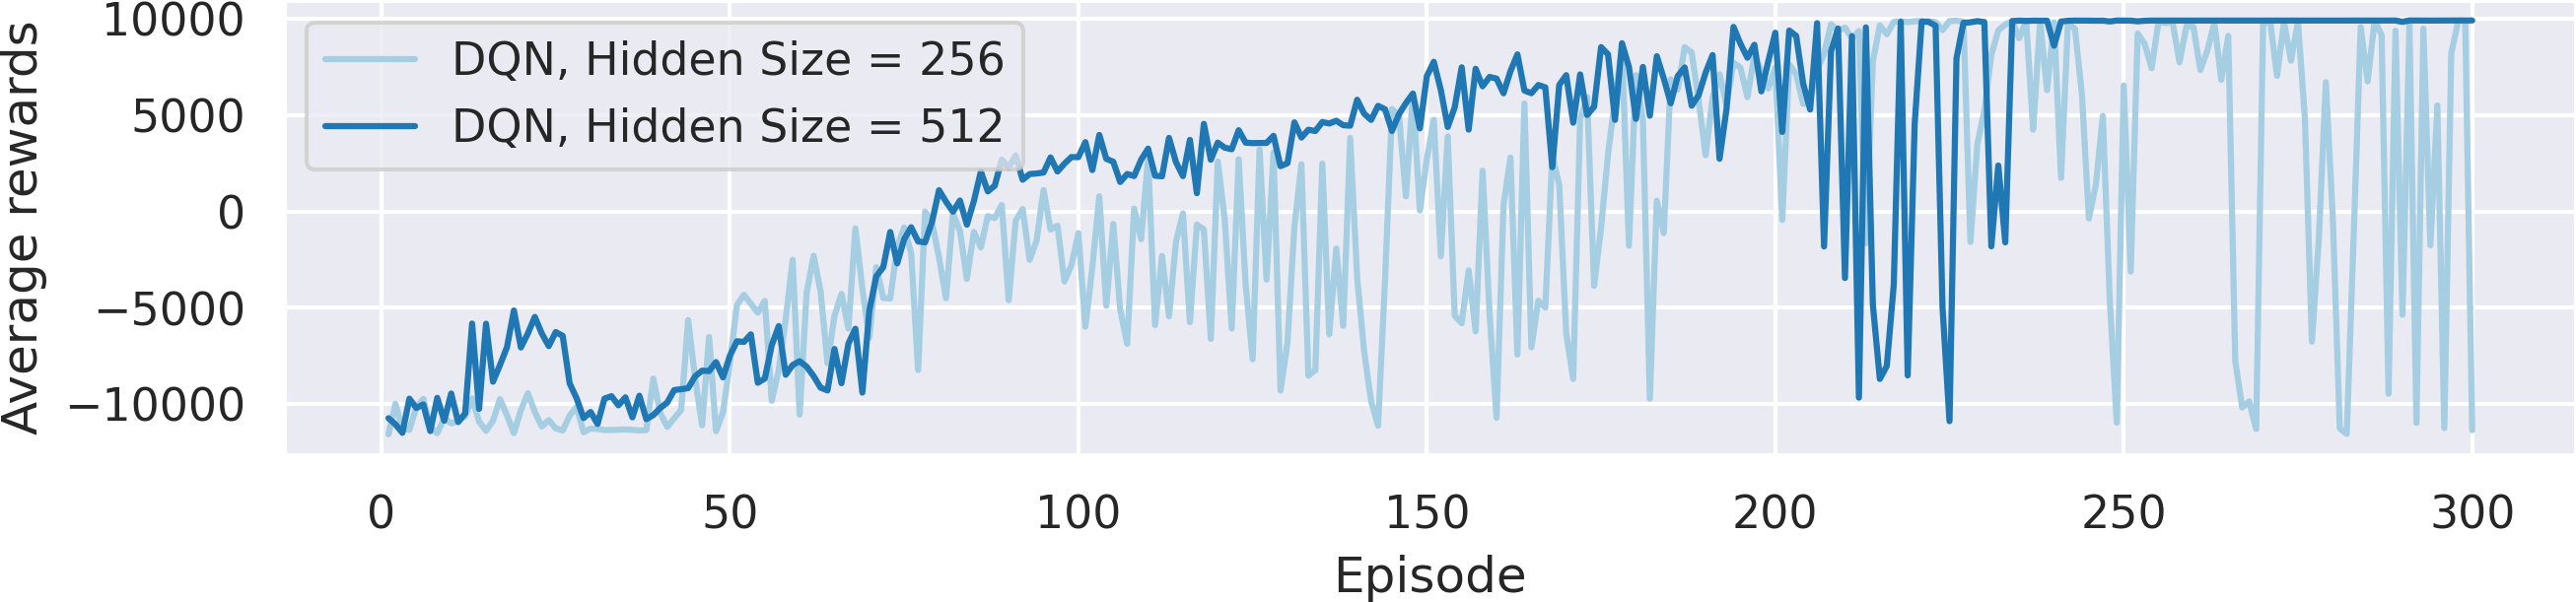
\includegraphics[width=\textwidth]{dqn_reward_size.png}
		\caption{Models using DQN.}
		\label{dqn_avg_reward}
	\end{subfigure} \\[1ex]
	\begin{subfigure}{\textwidth}
		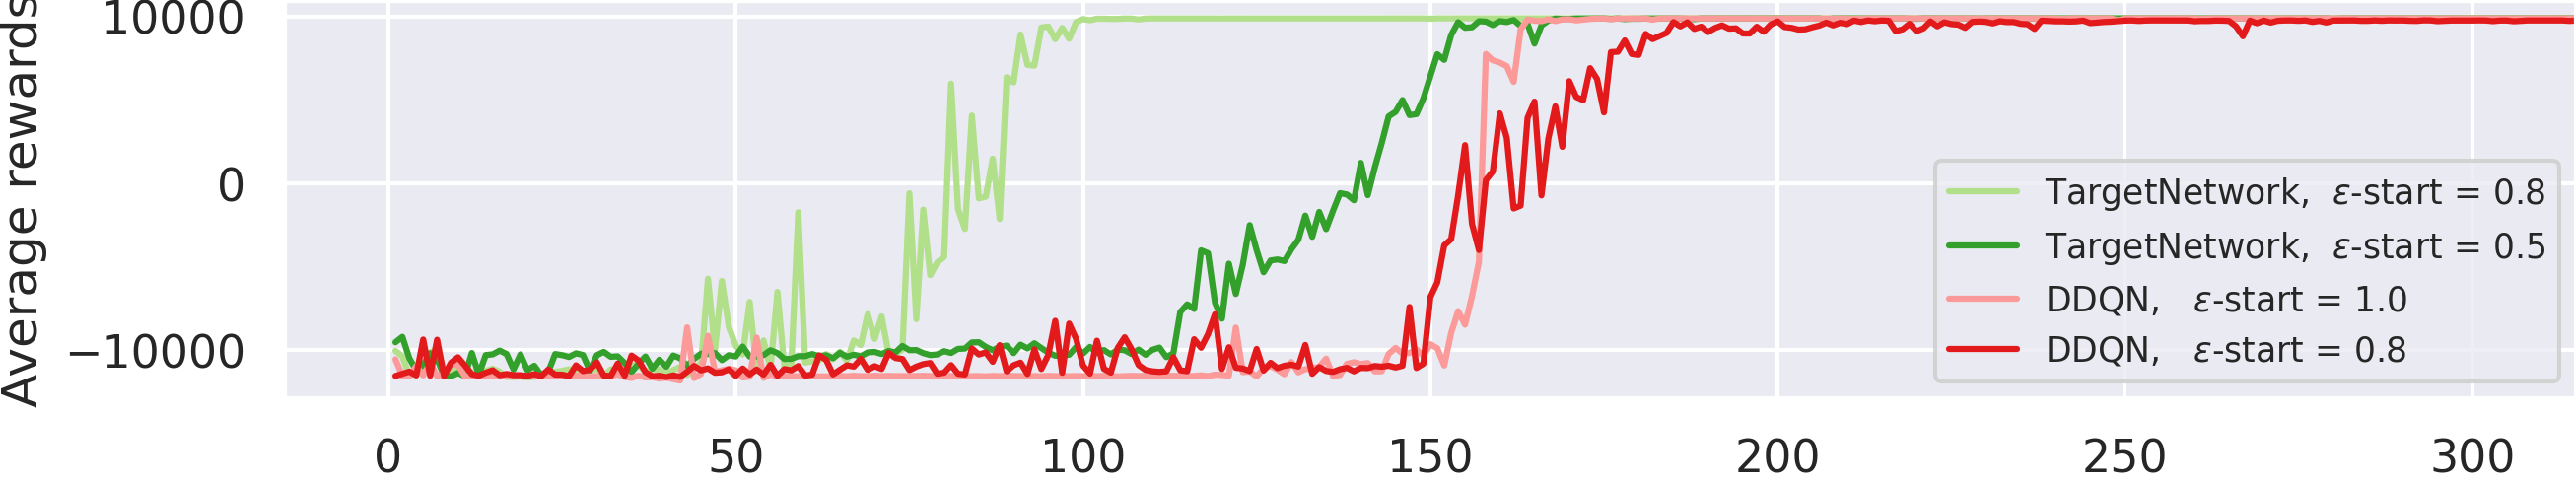
\includegraphics[width=\textwidth]{rest_reward_size.png}
		\caption{Models using DDQN and Target Network.}
		\label{rest_avg_reward}
	\end{subfigure}
	\caption{Reward sizes for the models presented in \cref{best_results_t2}.}
	\label{avg_reward}
\end{figure}

As seem in \cref{losses}, the loss of all models goes down in time except for the DDQN with $\varepsilon\text{-start} = 1.0$, whose loss shoots up and only comes down when the model converges.
The cause for this effect is difficult to find out, but it's likely chaos with the target network.
\begin{figure}[h]
	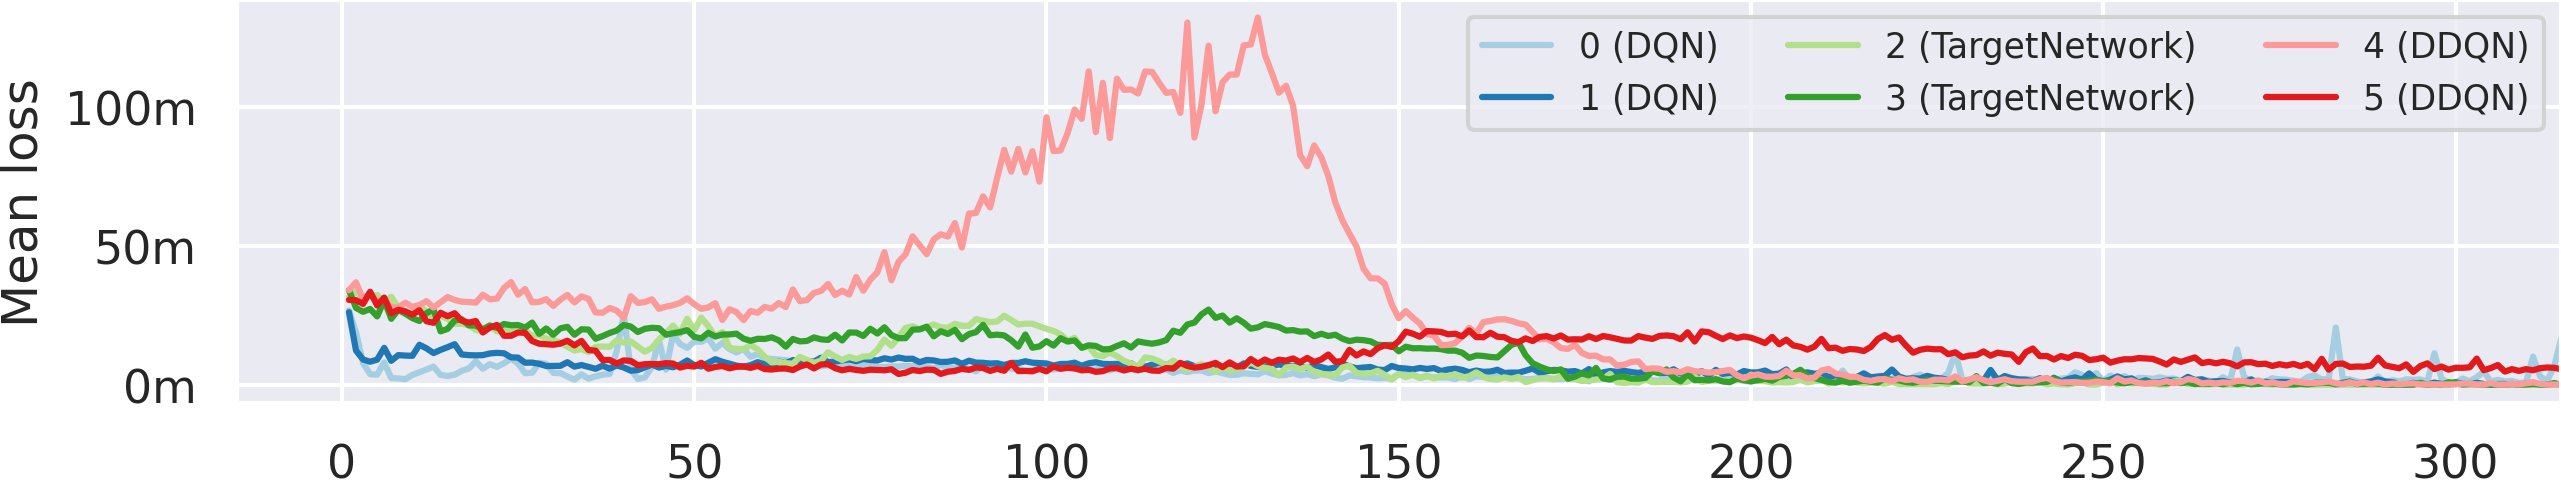
\includegraphics[width=\textwidth]{losses.png}
	\caption{Average loss of each model at each episode, with the mysterious loss spike for the DDQN with ID 4.}
	\label{losses}
\end{figure}

The expected Q values at each train, shown in \cref{q_values}, show a good example of the stability of the models: the ones for DDQN are smoother than the ones using TargetNetwork, which are smoother than the ones using DQN.
Interestingly, the target Q value follows the same spike as the loss in \cref{losses} and it's its likely cause.
\begin{figure}[h]
	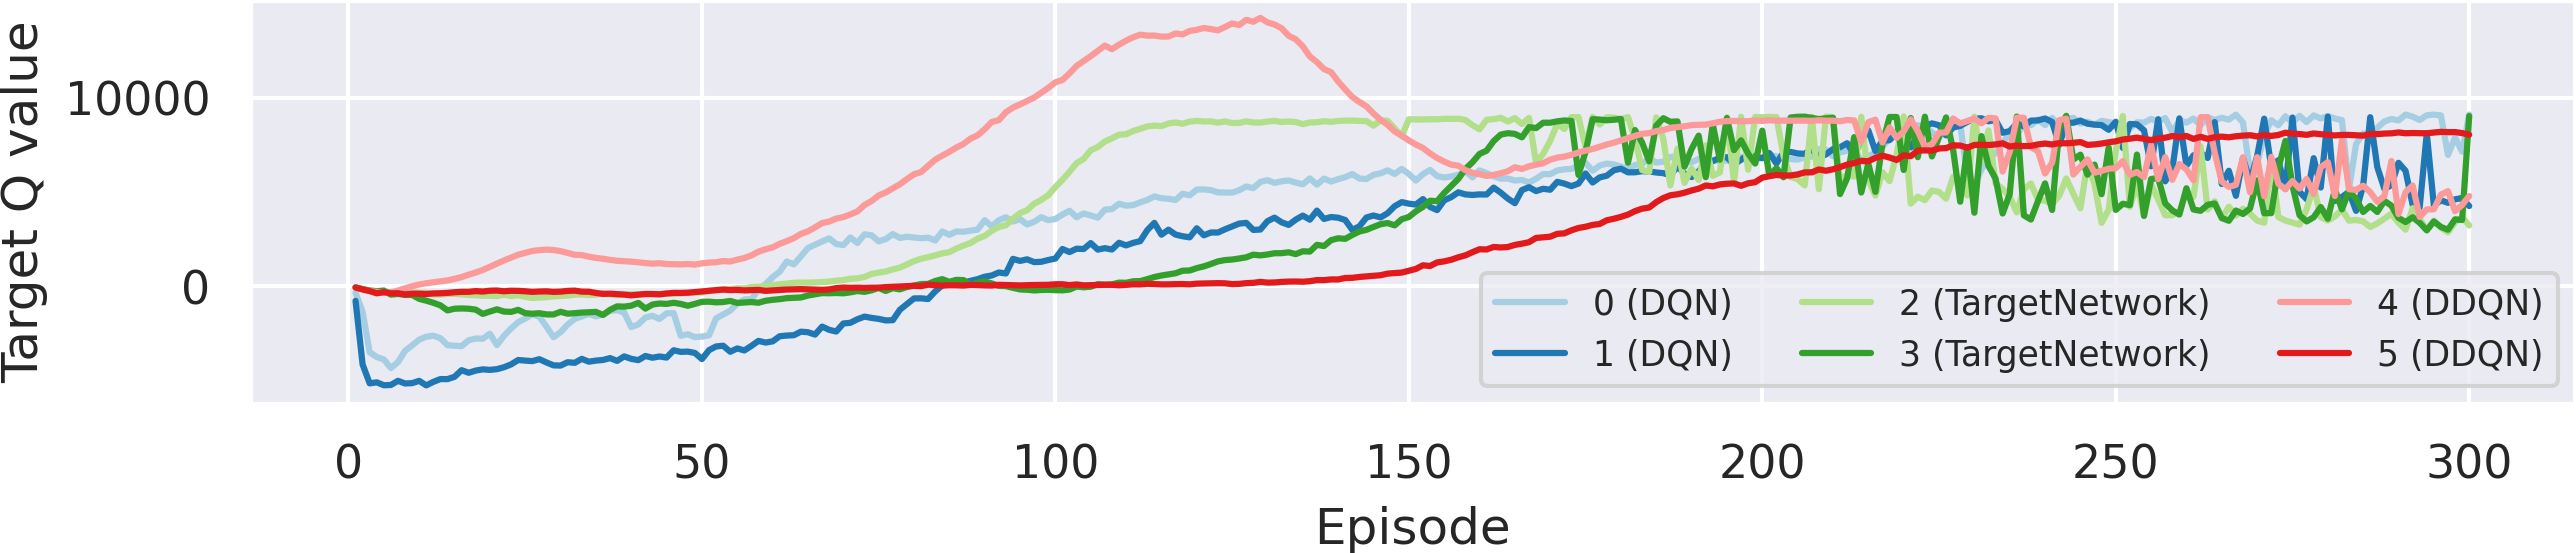
\includegraphics[width=\textwidth]{q_values.png}
	% \caption{Mean expected Q values of the models per episode.}
	\label{q_values}
\end{figure}

\newpage{}
\subsection{Qualitative Analysis}

However, what does it mean for a candidate to be better than another?

\Cref{circle_plots} shows 4 examples of the model with ID = 1 in \cref{best_results_t2} at different training episodes.
At each one of these episodes, 10 skaters are thrown in the environment with the objective of reaching the centre in as little time as possible.
These are validation skaters that use the model alone and are unaffected by $\varepsilon$.

\begin{figure}[H]
	\begin{subfigure}[t]{.48\textwidth}
		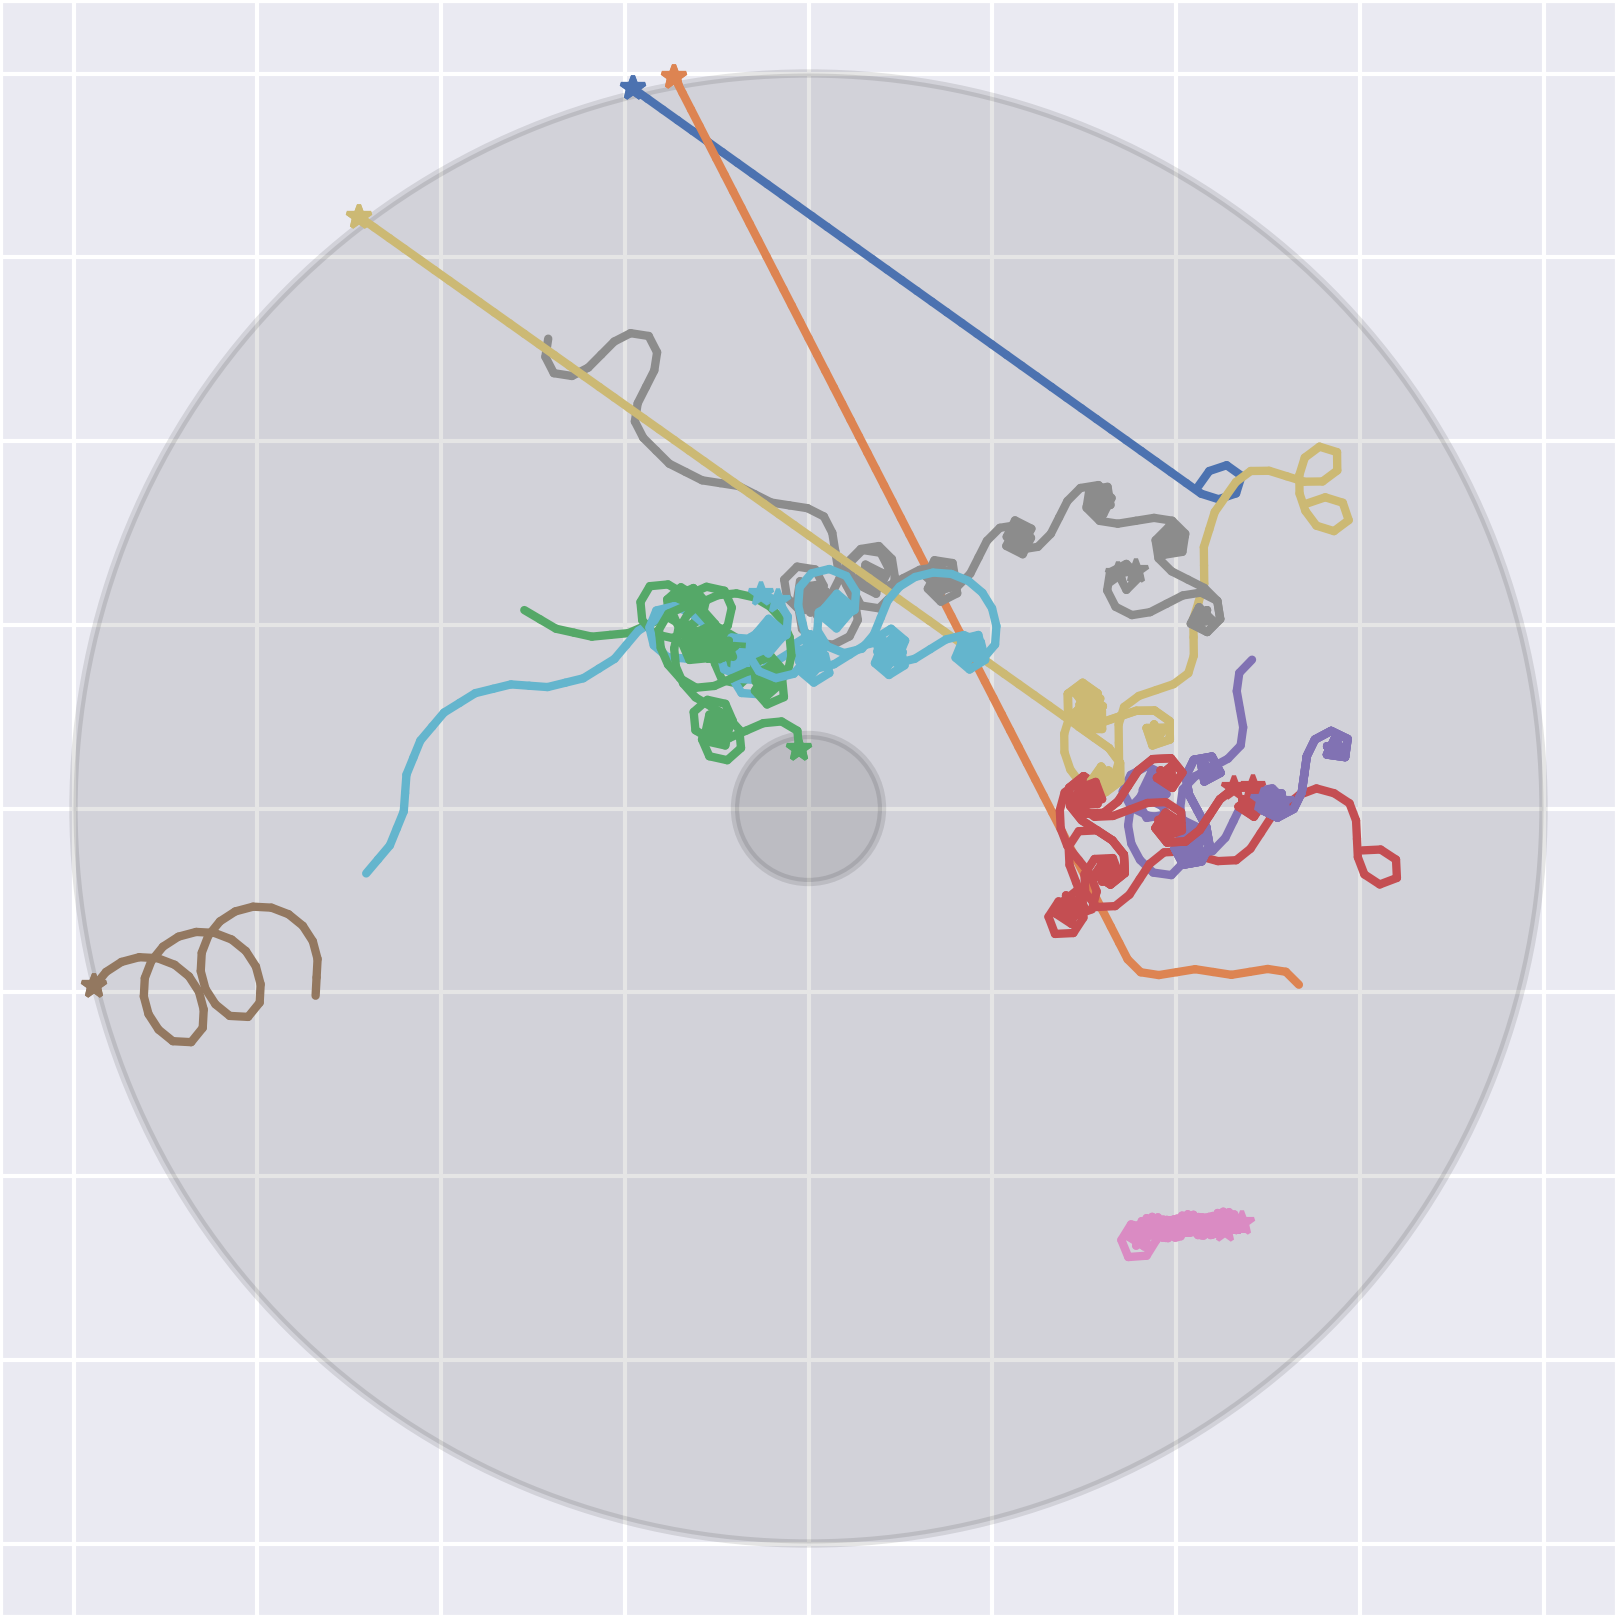
\includegraphics[width=\textwidth]{circle_images/image_50.png}
		\caption{State of the learners after \textbf{50 episodes}. The skaters act without much of a pattern, but there is one that reached the objective in the centre. Luck or intelligence?}
	\end{subfigure}\hfill{}
	\begin{subfigure}[t]{.48\textwidth}
		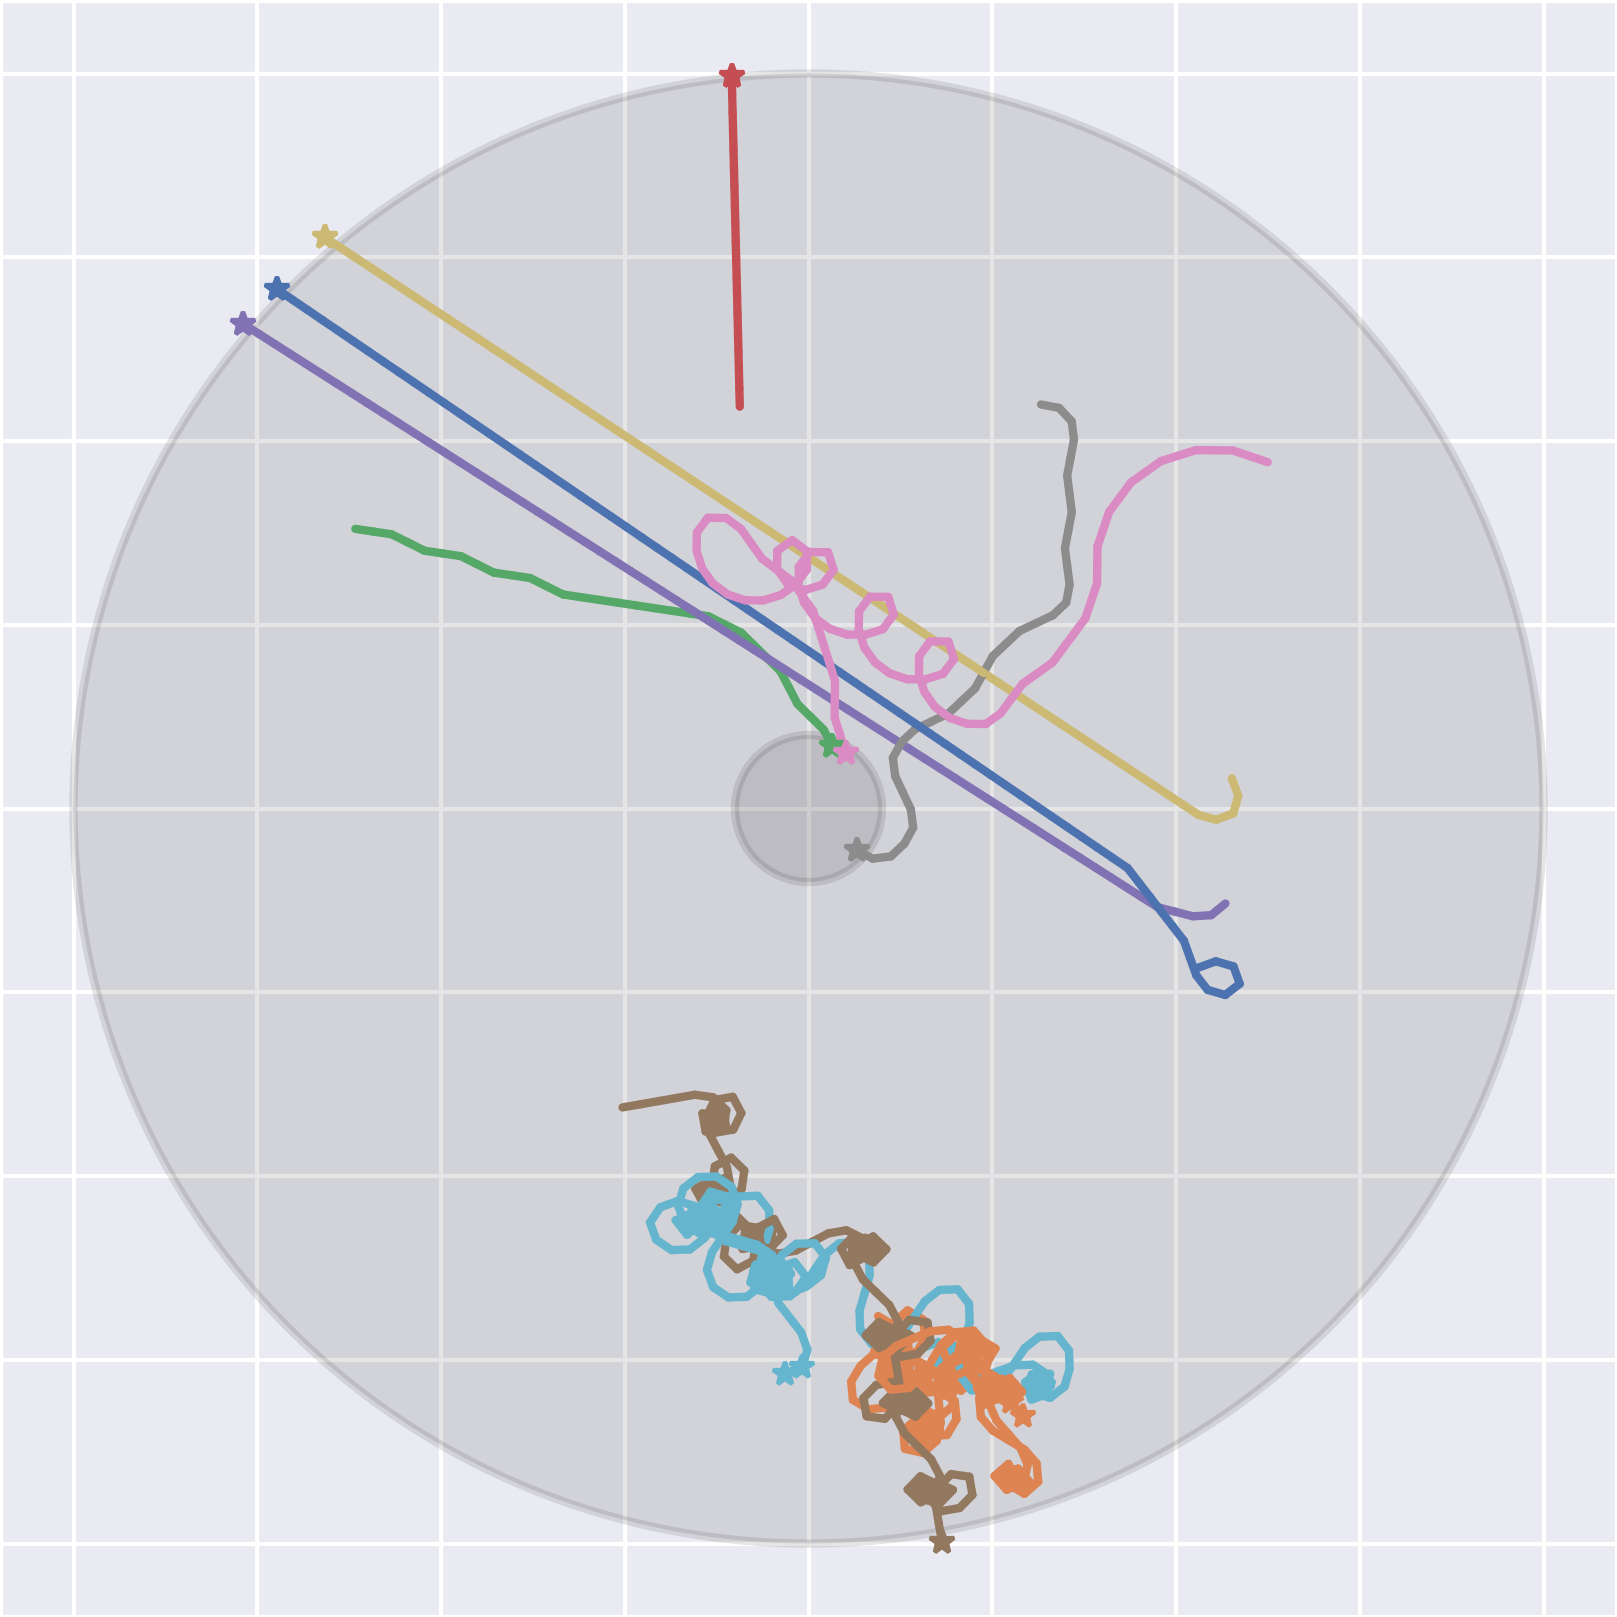
\includegraphics[width=\textwidth]{circle_images/image_100_alt_2.png}
		\caption{State of the learners after \textbf{100 episodes}. Skaters travel in a not-necessarily-straight path to the centre if they are close, or basically random if they are far. Additionally, some agents pass close to the centre but do not turn towards it.}
	\end{subfigure} \\
	\begin{subfigure}[t]{.48\textwidth}
		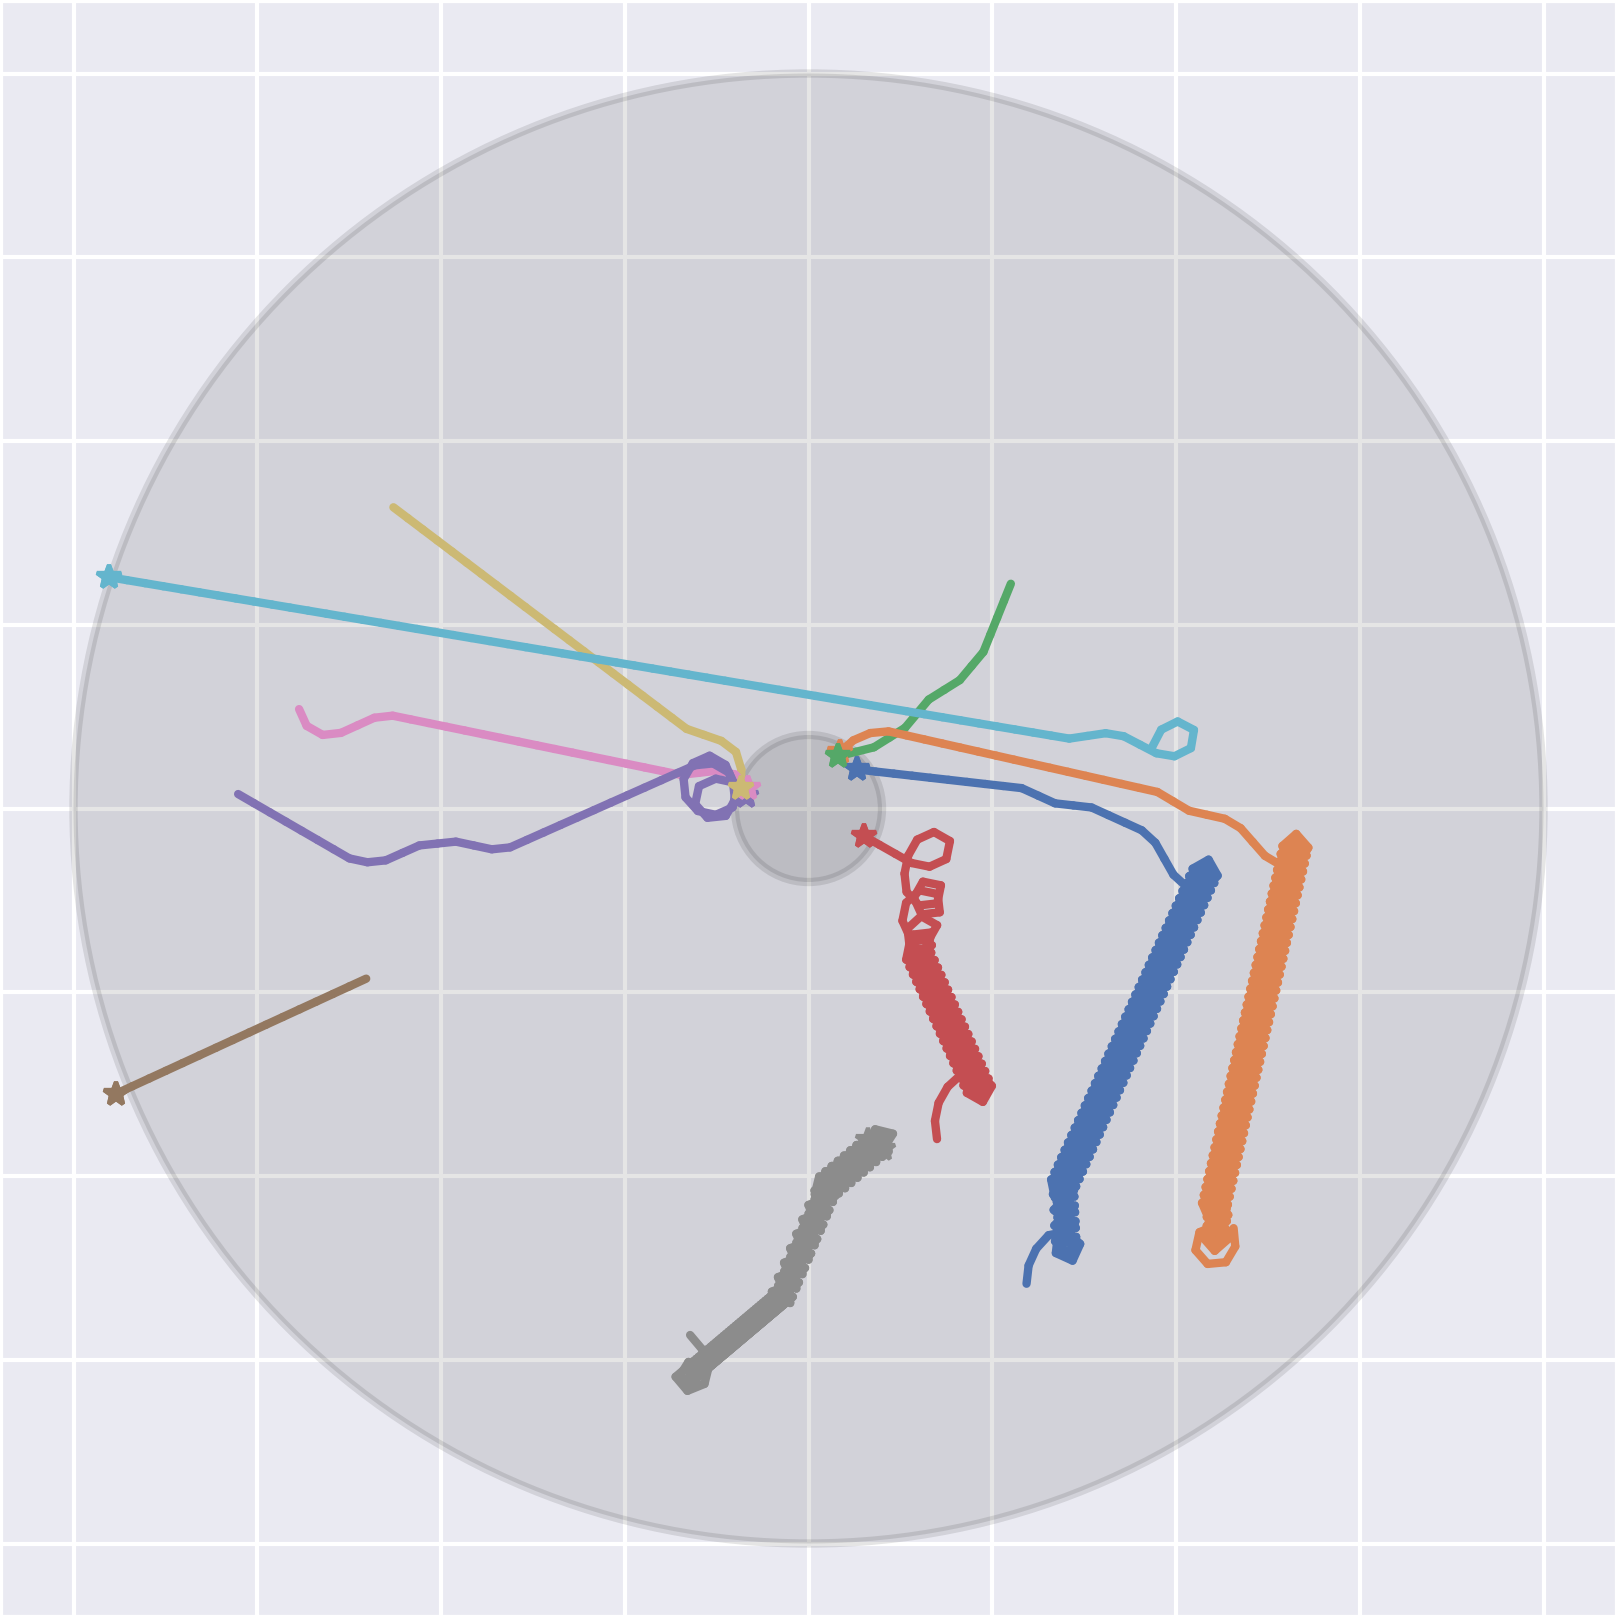
\includegraphics[width=\textwidth]{circle_images/image_150.png}
		\caption{State of the learners after \textbf{150 episodes}. Most skaters reach the centre, even if some of them get desperate their angular velocity at first, affecting their score.}
	\end{subfigure}\hfill{}
	\begin{subfigure}[t]{.48\textwidth}
		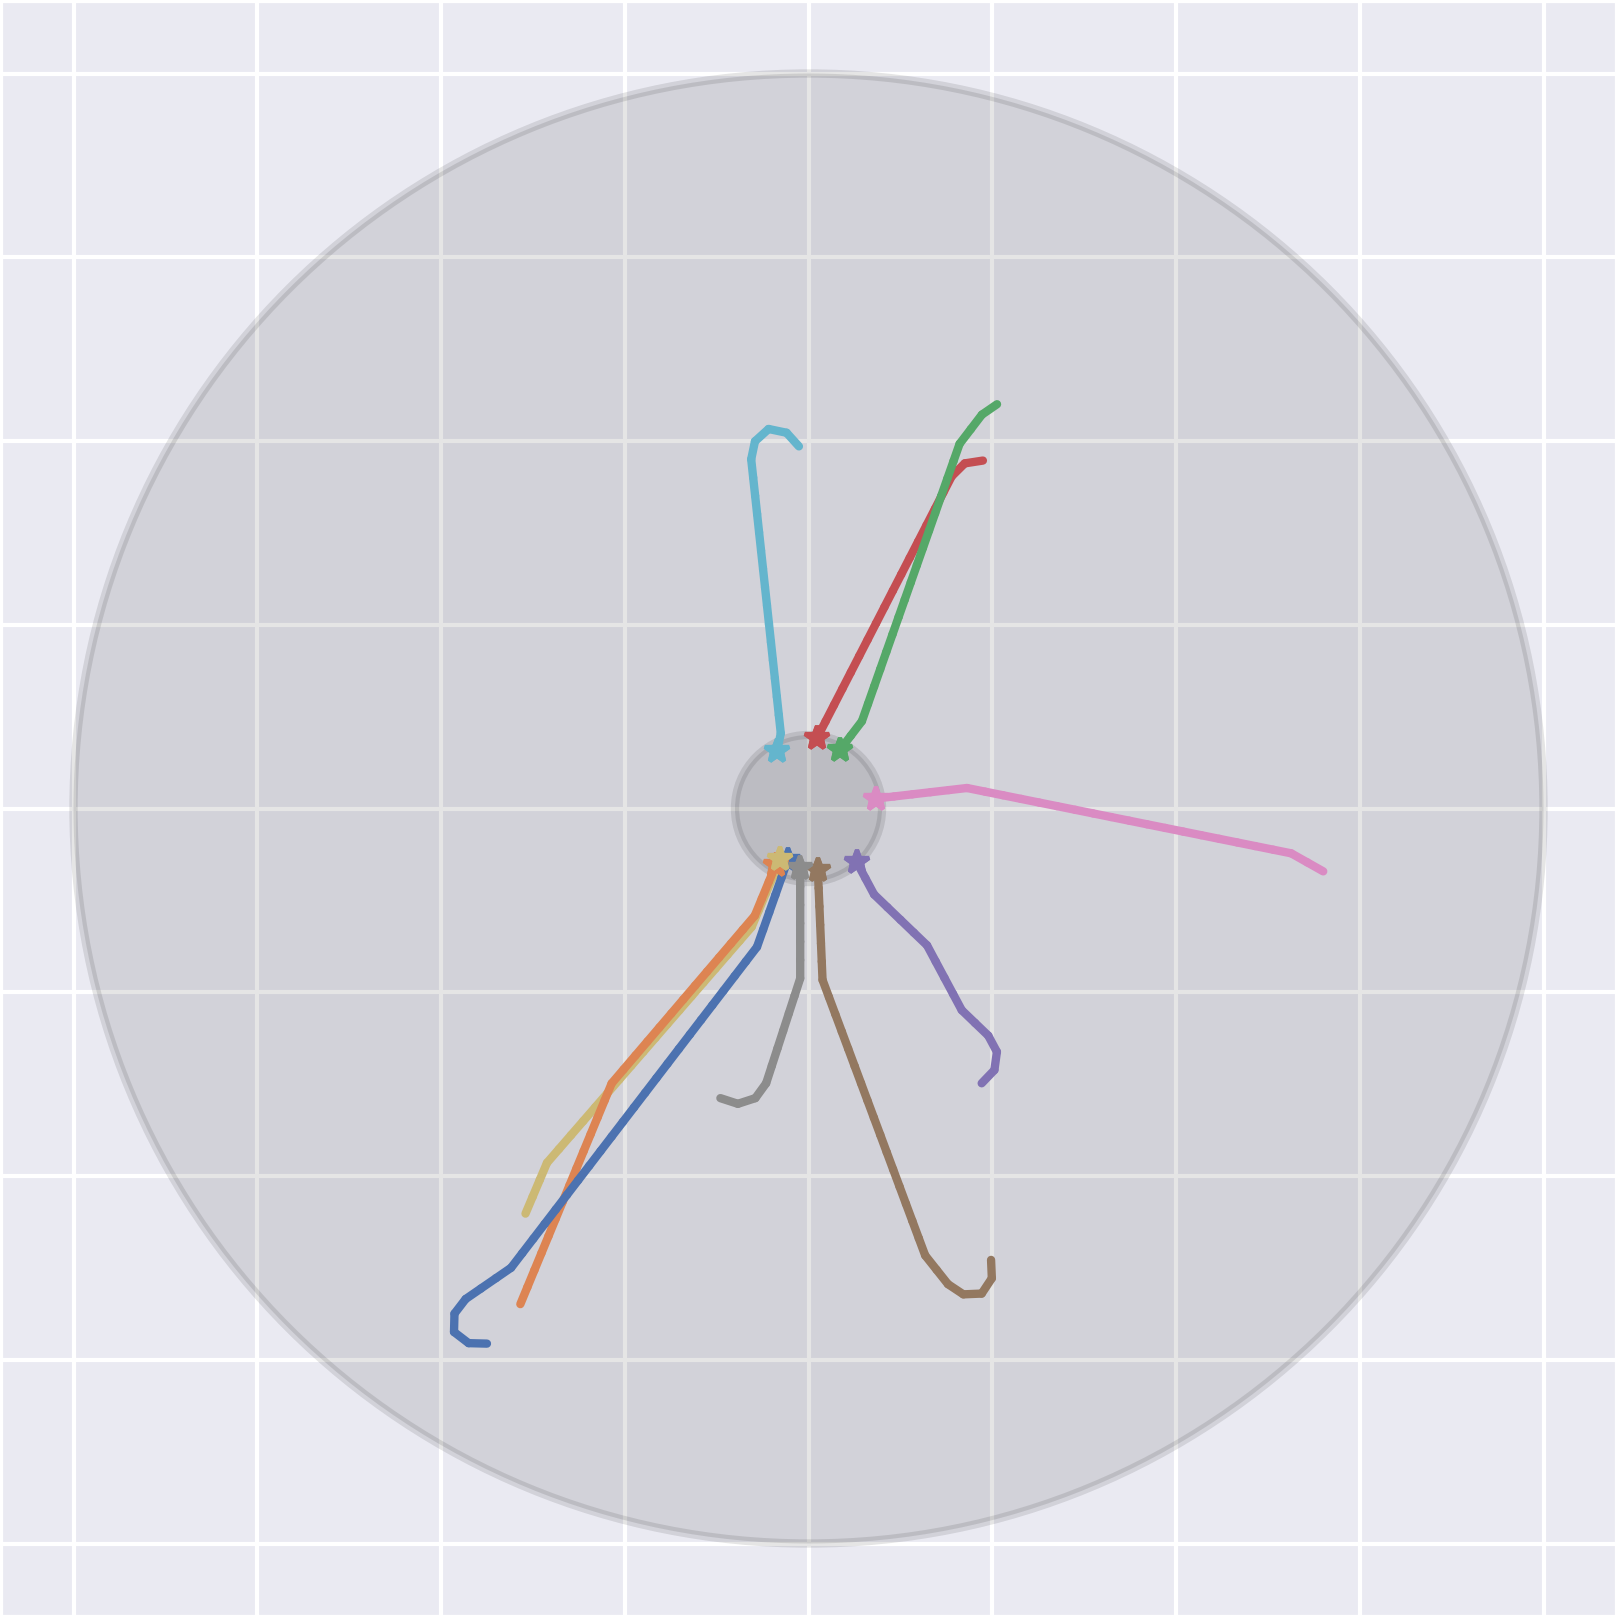
\includegraphics[width=\textwidth]{circle_images/image_300.png}
		\caption{After \textbf{300 episodes}, the skaters always find the shortest path to the centre regardless of where they start or in which direction they initially face.}
	\end{subfigure}
	\caption{Ice skating ice skating using DQN with hidden size = 512 (model \colorbox{id1}{1} in \cref{best_results_t2}).}
	\label{circle_plots}
\end{figure}


\section{RLLib}


\clearpage{}

\renewcommand{\thesection}{Extra Task}
\section{PPO Implementation}

For this section we attempt to implement Proximal Policy Optimization (PPO) where it deviates from the standard value-iteration calculations of the q-values used from techniques in the tasks above, and instead implements a policy gradient-based calculation. It implements a policy network and a value network. 

The PPO algorithm directly modifies the policy instead of the conventional state-action pairs obtained through the DQN methods. It utilises entropy and interactions with the environment to update the best policy for the agent to carry out to best fit the environment.

For the implementation, the code is referenced from the labs and also mildly inspired from the Atari PPO implementation\cite{ppo_github}, the environment used for this implementation is Space Invaders. The environment is modified to provide batches of input determined by batch size, followed by preprocessing techniques such as grayscaling and resizing to dimensions $84 \times 84$.

To learn the RGB image of the environment, the model is modified from taking discrete observation spaces as input to instead take in images through the addition of convolutional layers, flattened into dense layers to return an output. The output layers meanwhile, are modified to return two outputs, the predicted action determined by a softmax layer, followed by a value output to be calculated in the loss function.

The loss function is calculated as follows:
\begin{align*}
   L(\theta) = \mathbb{E}_t \left[ \min \left( r_t(\theta) \hat{A}_t, \text{clip}(r_t(\theta), 1 - \epsilon, 1 + \epsilon) \hat{A}_t \right) - \beta H(\pi_{\theta}) \right] 
\end{align*}

\subsection{Results}
Implementation of the PPO algorithm on Space Invaders sees a max reward of around 600 from a measly 105 over 600 episodes. This is a significant improvement over regular DQN methods.


\renewcommand{\thesection}{Individual Contribution}
\section{Individual Reflection}
Me and Martin have worked in tandem to contribute to this project equally. I have provided ideas for most of the algorithms and implemented the DDQN and Target Network methods and the extra task, while Martin has mostly contributed to the environment parameters itself and the implementation of the DQN. However, to say I did this and he did that would be unfair, as we have always sat down and worked together to complete this entire project. All in all, I am satisfied with my and Martin's contributions and I believe he agrees too.
\clearpage{}

\begin{appendices}
	\renewcommand{\topfraction}{1}
\renewcommand{\bottomfraction}{1}
\renewcommand{\textfraction}{0}
\renewcommand{\floatpagefraction}{1}

\renewcommand{\thesection}{Appendix A}
\section{Results of Parameter Sweep for Task 1}
\label{param_sweep_result_appendix}

\begin{table}[h]
	\scriptsize
	\centering
	\begin{tabular}{r l r | r r r r}
		\toprule
		$\alpha$ & $\gamma$ & $\epsilon$ Decay &
		E.\ to Conv & Best route & E.\ to Done & E.\ to Best\footnotemark[0]{} \\
		\midrule
		0.2  & 0.90  & 0.75 & 335 & 17.80 & 62.10  & 116 \\
		0.2  & 0.90  & 0.90 & 328 & 17.20 & 60.00  & 119 \\
		0.2  & 0.90  & 0.99 & 314 & 16.00 & 40.90  & 100 \\
		0.2  & 0.99  & 0.75 & 794 & 18.00 & 509.80 & 334 \\
		0.2  & 0.99  & 0.90 & 915 & 17.50 & 597.50 & 1621 \\
		0.2  & 0.99  & 0.99 & 406 & 16.30 & 102.70 & 157 \\
		0.5  & 0.90  & 0.75 & 125 & 17.40 & 28.60  & 48 \\
		0.5  & 0.90  & 0.90 & 111 & 17.00 & 15.30  & 31 \\
		\rowcolor{YellowGreen}
		0.5  & 0.90  & 0.99 & 139 & 16.00 & 31.80  & 97 \\
		0.5  & 0.99  & 0.75 & 259 & 18.20 & 157.70 & 186 \\
		0.5  & 0.99  & 0.90 & 262 & 17.00 & 160.40 & 212 \\
		0.5  & 0.99  & 0.99 & 176 & 16.00 & 49.70  & 114 \\
		0.7  & 0.90  & 0.75 & 79  & 17.10 & 17.70  & 55 \\
		0.7  & 0.90  & 0.90 & 78  & 16.40 & 16.10  & 29 \\
		0.7  & 0.90  & 0.99 & 111 & 16.30 & 26.10  & 93 \\
		0.7  & 0.99  & 0.75 & 193 & 17.50 & 123.10 & 144 \\
		0.7  & 0.99  & 0.90 & 178 & 18.00 & 111.70 & None \\
		0.7  & 0.99  & 0.99 & 133 & 16.10 & 44.30  & 111 \\
		0.9 & 0.90  & 0.75 & 53  & 17.30 & 15.20  & 41 \\
		0.9 & 0.90  & 0.90 & 51  & 16.80 & 12.00  & 26 \\
		0.9 & 0.90  & 0.99 & 81  & 17.50 & 22.10  & 75 \\
		0.9 & 0.99  & 0.75 & 147 & 18.60 & 106.50 & 189 \\
		0.9 & 0.99  & 0.90 & 158 & 18.20 & 108.40 & 72 \\
		0.9 & 0.99  & 0.99 & 113 & 16.50 & 46.80  & 111 \\
		\bottomrule
	\end{tabular}
	\caption{Parameter Sweep using $\epsilon$-Greedy policy.}
	\vspace{3em}
	\begin{tabular}{r l r | r r r r}
		$\alpha$ & $\gamma$ & $\epsilon$ Decay &
		E.\ to Conv & Best route & E.\ to Done & E.\ to Best\footnotemark[0]{} \\
		\midrule
			0.2 & 0.90 & 0.75 & 666  & 16.20 &  82.70 &  224 \\
			0.2 & 0.90 & 0.90 & 682  & 16.20 & 130.00 &  247 \\
			0.2 & 0.90 & 0.99 & 625  & 16.70 & 107.90 &  205 \\
			0.2 & 0.99 & 0.75 & 1371 & 16.60 & 498.00 &  556 \\
			0.2 & 0.99 & 0.90 & 1876 & 17.50 & 406.90 &  546 \\
			0.2 & 0.99 & 0.99 & 1347 & 17.20 & 419.00 &  726 \\
			0.5 & 0.90 & 0.75 & 288  & 17.40 &  79.70 &  148 \\
			0.5 & 0.90 & 0.90 & 293  & 17.20 &  80.90 &  121 \\
			0.5 & 0.90 & 0.99 & 252  & 16.50 &  50.80 &  114 \\
			0.5 & 0.99 & 0.75 & 617  & 17.20 &  273.6 &  620 \\
			0.5 & 0.99 & 0.90 & 550  & 17.40 &  96.30 &  278 \\
			0.5 & 0.99 & 0.99 & 810  & 17.10 & 432.60 &  533 \\
			0.7 & 0.90 & 0.75 & 205  & 17.60 &  48.70 &   58 \\
			0.7 & 0.90 & 0.90 & 192  & 18.00 &  44.10 &   83 \\
			0.7 & 0.90 & 0.99 & 196  & 17.60 &  56.20 &  122 \\
			0.7 & 0.99 & 0.75 & 453  & 17.40 & 222.30 &  382 \\
			0.7 & 0.99 & 0.90 & 415  & 17.20 & 157.00 &  175 \\
			0.7 & 0.99 & 0.99 & 612  & 17.90 & 228.00 &  300 \\
			0.9 & 0.90 & 0.75 & 149  & 17.40 &  50.20 &  107 \\
			0.9 & 0.90 & 0.90 & 129  & 17.20 &  39.30 &   53 \\
			0.9 & 0.90 & 0.99 & 126  & 17.40 &  37.30 &   86 \\
			0.9 & 0.99 & 0.75 & 272  & 23.70 &  85.20 & None \\
			0.9 & 0.99 & 0.90 & 258  & 36.75 &  97.25 & None \\
			0.9 & 0.99 & 0.99 & 266  & 24.80 & 128.10 &  185 \\
		\bottomrule
	\end{tabular}
	\caption{Parameter Sweep using Bellman policy.}
\end{table}


\footnotetext{This is the average amount of epochs until it finds the absolute best value for batches that find it in any of the 10 repetitions, or None if this is never found.}

	\clearpage{}
	\renewcommand{\topfraction}{1}
\renewcommand{\bottomfraction}{1}
\renewcommand{\textfraction}{0}
\renewcommand{\floatpagefraction}{1}

\renewcommand{\thesection}{Appendix B}
\section{Results of Parameter Sweep for Task 2}
\label{param_sweep_result_appendix_task2}

\begin{table}[h]
	\centering
	\scriptsize
	\begin{tabular}{r r r r | r r r r r r}
		\toprule
			hidden size & lr & gamma & eps start & win rate & best episode & best dones & loss & q step \\
		\midrule
			256 & 0.001 & 0.9 & 1 & 0.987 & 44 & 1000 & 24035k & -786.76 \\
			256 & 0.001 & 0.9 & 0.8 & 0.115 & 499 & 990 & 7429k & -326.81 \\
			256 & 0.001 & 0.9 & 0.5 & 0.042 & 441 & 954 & 8409k & 344.73 \\
			256 & 0.001 & 0.99 & 1 & 0 & 374 & 1000 & 8577k & 5293.25 \\
			256 & 0.001 & 0.99 & 0.8 & 1 & 257 & 1000 & 2078k & 7717.68 \\
			256 & 0.001 & 0.99 & 0.5 & 1 & 178 & 1000 & 10030k & 7091.87 \\
			256 & 0.0001 & 0.9 & 1 & 0.009 & 28 & 1000 & 31225k & -1254.27 \\
			256 & 0.0001 & 0.9 & 0.8 & 0.324 & 33 & 1000 & 30087k & -1211.92 \\
			256 & 0.0001 & 0.9 & 0.5 & 0.171 & 324 & 715 & 42532k & -881.39 \\
			256 & 0.0001 & 0.99 & 1 & 0 & 353 & 743 & 11764k & -4141.98 \\
			256 & 0.0001 & 0.99 & 0.8 & 0.925 & 375 & 937 & 18652k & -2407.15 \\
			256 & 0.0001 & 0.99 & 0.5 & 0.733 & 497 & 955 & 6749k & 6657.05 \\
			512 & 0.001 & 0.9 & 1 & 1 & 404 & 1000 & 4546k & 3569.51 \\
			512 & 0.001 & 0.9 & 0.8 & 0.053 & 493 & 964 & 16321k & -577.39 \\
			512 & 0.001 & 0.9 & 0.5 & 0.995 & 417 & 1000 & 2164k & 3995.84 \\
			512 & 0.001 & 0.99 & 1 & 1 & 259 & 1000 & 2342k & 7443.32 \\
			512 & 0.001 & 0.99 & 0.8 & 1 & 197 & 1000 & 8306k & 4608.34 \\
			512 & 0.001 & 0.99 & 0.5 & 0.03 & 181 & 1000 & 1708k & 7621.50 \\
			512 & 0.0001 & 0.9 & 1 & 0.403 & 41 & 1000 & 32119k & -1251.44 \\
			512 & 0.0001 & 0.9 & 0.8 & 0.227 & 46 & 920 & 24237k & -1108.12 \\
			512 & 0.0001 & 0.9 & 0.5 & 0.112 & 33 & 882 & 23551k & -1118.50 \\
			512 & 0.0001 & 0.99 & 1 & 0.014 & 30 & 736 & 10707k & -5260.23 \\
			512 & 0.0001 & 0.99 & 0.8 & 1 & 433 & 1000 & 14180k & 7158.44 \\
			512 & 0.0001 & 0.99 & 0.5 & 0.17 & 129 & 625 & 8532k & -855.20 \\
		\bottomrule
	\end{tabular}
	\caption{Results using DQN.}
	\label{dqn_results}
\end{table}

\begin{table}[h]
	\centering
	\scriptsize
	\begin{tabular}{r r r r | r r r r r r}
		\toprule
			hidden size & lr & gamma & eps start & win rate & best episode & best dones & loss & q step \\
		\midrule
			256 & 0.001 & 0.9 & 1 & 1 & 312 & 1000 & 12210k & 3793.82 \\
			256 & 0.001 & 0.9 & 0.8 & 1 & 333 & 1000 & 10719k & 3606.29 \\
			256 & 0.001 & 0.9 & 0.5 & 0.051 & 29 & 603 & 26203k & -166.52 \\
			256 & 0.001 & 0.99 & 1 & 1 & 174 & 1000 & 15189k & 7121.94 \\
			256 & 0.001 & 0.99 & 0.8 & 1 & 288 & 1000 & 14735k & 6244.03 \\
			256 & 0.001 & 0.99 & 0.5 & 1 & 481 & 1000 & 7323k & 7309.51 \\
			256 & 0.0001 & 0.9 & 1 & 0.019 & 41 & 922 & 29113k & -143.43 \\
			256 & 0.0001 & 0.9 & 0.8 & 0.023 & 173 & 935 & 36930k & -147.35 \\
			256 & 0.0001 & 0.9 & 0.5 & 0.025 & 102 & 1000 & 38872k & -160.46 \\
			256 & 0.0001 & 0.99 & 1 & 0.003 & 27 & 378 & 25732k & -1322.65 \\
			256 & 0.0001 & 0.99 & 0.8 & 0 & 35 & 266 & 18097k & -1318.79 \\
			256 & 0.0001 & 0.99 & 0.5 & 0.021 & 205 & 707 & 20555k & -638.11 \\
			512 & 0.001 & 0.9 & 1 & 1 & 224 & 1000 & 21838k & 3133.20 \\
			512 & 0.001 & 0.9 & 0.8 & 1 & 335 & 1000 & 8756k & 3891.60 \\
			512 & 0.001 & 0.9 & 0.5 & 0.631 & 483 & 682 & 23161k & -11.06 \\
			512 & 0.001 & 0.99 & 1 & 1 & 162 & 1000 & 20004k & 7219.42 \\
			\rowcolor{YellowGreen}
			512 & 0.001 & 0.99 & 0.8 & 1 & 94 & 1000 & 17494k & 6114.58 \\
			512 & 0.001 & 0.99 & 0.5 & 1 & 124 & 1000 & 12819k & 6709.36 \\
			512 & 0.0001 & 0.9 & 1 & 0.006 & 46 & 830 & 25243k & -101.25 \\
			512 & 0.0001 & 0.9 & 0.8 & 0.022 & 80 & 802 & 25421k & -151.95 \\
			512 & 0.0001 & 0.9 & 0.5 & 0.115 & 36 & 947 & 26183k & -156.47 \\
			512 & 0.0001 & 0.99 & 1 & 0 & 28 & 617 & 22347k & -1127.83 \\
			512 & 0.0001 & 0.99 & 0.8 & 0.011 & 35 & 468 & 17002k & -1077.71 \\
			512 & 0.0001 & 0.99 & 0.5 & 0.018 & 37 & 903 & 26250k & -798.06 \\
		\bottomrule
	\end{tabular}
	\caption{Results using target network method.}
	\label{targetnetwork_results}
\end{table}

\begin{table}[h]
	\centering
	\scriptsize
	\begin{tabular}{r r r r | r r r r r r}
		\toprule
			hidden size & lr & gamma & eps start & win rate & best episode & best dones & loss & q step \\
		\midrule
			256 & 0.001 & 0.9 & 1 & 1 & 245 & 1000 & 14873k & 3271.52 \\
			256 & 0.001 & 0.9 & 0.8 & 1 & 215 & 1000 & 28020k & 2325.41 \\
			256 & 0.001 & 0.9 & 0.5 & 0.989 & 473 & 1000 & 5157k & 3946.32 \\
			256 & 0.001 & 0.99 & 1 & 1 & 185 & 1000 & 16965k & 6043.44 \\
			256 & 0.001 & 0.99 & 0.8 & 1 & 129 & 1000 & 18415k & 5516.58 \\
			256 & 0.001 & 0.99 & 0.5 & 1 & 253 & 1000 & 15840k & 7333.18 \\
			256 & 0.0001 & 0.9 & 1 & 0.017 & 53 & 852 & 27453k & -124.09 \\
			256 & 0.0001 & 0.9 & 0.8 & 0.011 & 155 & 1000 & 22849k & -170.79 \\
			256 & 0.0001 & 0.9 & 0.5 & 0.018 & 107 & 1000 & 32784k & -155.53 \\
			256 & 0.0001 & 0.99 & 1 & 0 & 39 & 328 & 21263k & -1415.99 \\
			256 & 0.0001 & 0.99 & 0.8 & 0.035 & 26 & 365 & 19274k & -1274.84 \\
			256 & 0.0001 & 0.99 & 0.5 & 0.035 & 156 & 749 & 24424k & -420.54 \\
			512 & 0.001 & 0.9 & 1 & 0.991 & 270 & 1000 & 14161k & 3634.89 \\
			512 & 0.001 & 0.9 & 0.8 & 1 & 250 & 1000 & 15151k & 3764.64 \\
			512 & 0.001 & 0.9 & 0.5 & 0.826 & 480 & 883 & 4878k & 789.87 \\
			512 & 0.001 & 0.99 & 1 & 1 & 101 & 1000 & 22431k & 4119.00 \\
			512 & 0.001 & 0.99 & 0.8 & 1 & 107 & 1000 & 13977k & 7215.91 \\
			512 & 0.001 & 0.99 & 0.5 & 1 & 157 & 1000 & 8232k & 8102.60 \\
			512 & 0.0001 & 0.9 & 1 & 0.275 & 39 & 867 & 35166k & -139.16 \\
			512 & 0.0001 & 0.9 & 0.8 & 0.017 & 86 & 698 & 27821k & -124.80 \\
			512 & 0.0001 & 0.9 & 0.5 & 0.002 & 75 & 895 & 25326k & -130.96 \\
			512 & 0.0001 & 0.99 & 1 & 0 & 26 & 105 & 28365k & -1373.54 \\
			512 & 0.0001 & 0.99 & 0.8 & 1 & 290 & 1000 & 29926k & 5529.61 \\
			512 & 0.0001 & 0.99 & 0.5 & 1 & 305 & 1000 & 47283k & 6504.88 \\
		\bottomrule
	\end{tabular}
	\caption{Result using double DQN.}
	\label{ddqn_results}
\end{table}

	\clearpage{}
	\renewcommand{\thesection}{Appendix C}
\renewcommand{\thesubsection}{}
\section{Source Code}

\subsection{Basic Task}
\lstinputlisting[title=Environment.py]{../Task 1/Environment.py}
\lstinputlisting[title=large\_map]{../Task 1/large_map}
\lstinputlisting[title=ice\_puzzle.py]{../Task 1/IcePuzzle.py}

\subsection{Advanced Task 1}
\lstinputlisting[title=SkatingRinkEnv.py]{../Task 2/SkatingRinkEnv.py}
\lstinputlisting[title=DQN.py]{../Task 2/DQN.py}
\lstinputlisting[title=Trainer.py]{../Task 2/Trainer.py}
\lstinputlisting[title=ReplayBuffer.py]{../Task 2/ReplayBuffer.py}
\lstinputlisting[title=rink.py]{../Task 2/rink.py}

\end{appendices}

\clearpage{}
\bibliography{reinforcement_report.bib}

\end{document}
